\documentclass{article}

\usepackage{amsmath}
\usepackage{amssymb}
\usepackage{url}
\usepackage{graphicx}
\usepackage{listings,color}
\usepackage{setspace}

\lstset{language=matlab,
        basicstyle=\ttfamily\scriptsize\singlespacing,
        keywordstyle=\color{blue},
        stringstyle=\color{red},
        commentstyle=\color{green},
        morecomment=[l][\color{magenta}]{\#},
        frame=L,
        xleftmargin=\parindent,
        numbersep=5pt,
        breaklines=true,
        breakatwhitespace=false,
        escapeinside={\%*}{*)},
}

\setlength{\parindent}{0cm}

\setlength{\parskip}{1mm}

\begin{document}

\title{\vspace{-2cm}Homework 3: Bidirectional Associative Memory}
\author{Andy Reagan}

\maketitle

\section{Discussion}

From exploring what BAM looks like from the state space, I've found that BAM, when stable, can only map memories to another node and then back to the start.
Also, starting at the other node, you have to get mapped back to memory that was stored on the other side, for it to be stable.
Otherwise there is no way for the weight matrix $W$ to encode the desired memories.

I'm still trying to make sense of how the weight matrix $W$ is set, but I've gotten this far: recalling the memory $B_1$ associated with $A_1$ goes like
\[ B_1 = f(A_1 W) = f(A_1 (A_1^TB_1 + \cdot A_n^TB_n)) = f(P_{A_1} B_1 + \cdot P_{A_1A_n}B_n) \]
where the $P_A$ is the projection matrix that projects $B$ on the basis of $A$.
The projection matrix for orthogonal vectors is 0, and the projection matrix of $A$ onto $A$ is the identity, so this will lead to perfect recall if the memories to be stored are indeed a basis of the vector space for their associations.

%% \begin{align*} 0 = -\frac{\epsilon}{h^2} + \frac{hf'''(x)}{3}\end{align*}

\section{Visualization}

I coded up the network in Javascript and made a force layout of the states of the network, drawing links as you move through the network.
I can show you (the class) a demo of it running, it's pretty fun.
The javascript code is attached, it also relies on a css and an html file which I didn't include.

Check it out live here: \url{http://andyreagan.github.io/demos/2015-02AANN/BAM.html}.

Starting at any given state in the network, the green dashed lines follow $W^T$, and the grey lines follow $W$.
It is sometimes tricky, but if you look closely it is always unambiguous how states are updated using these maps.

Here are a couple screen shots from it:

\begin{figure}[h!]
 \centering
  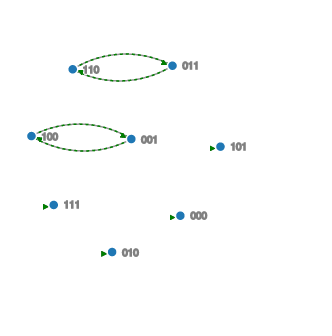
\includegraphics[width=0.69\textwidth]{network1.png}
  \label{fig:1}
  \caption{The network for the memories given in class.}
\end{figure}

\begin{figure}[h!]
 \centering
  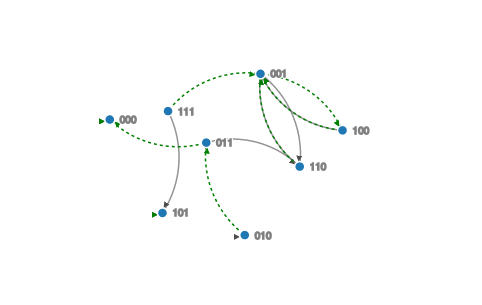
\includegraphics[width=0.79\textwidth]{network2.png}
  \label{fig:2}
  \caption{The network for the memories given in class, with a slight change so that the two memories are not symmetric. More interesting!}
\end{figure}

\begin{figure}[h!]
 \centering
  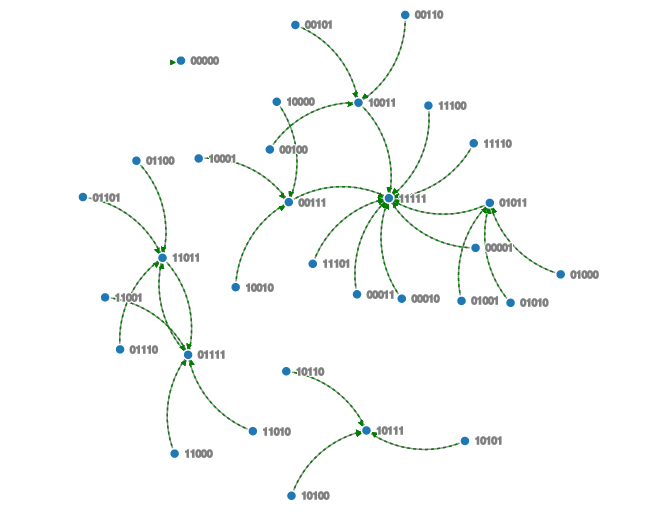
\includegraphics[width=0.79\textwidth]{network3.png}
  \label{fig:2}
  \caption{A bigger network having some trouble remembering things. Maybe I coded it wrong...}
\end{figure}

\clearpage
\pagebreak

\section*{Full code}

\lstinputlisting[]{bam_andy_driver.m}

\clearpage
\pagebreak

\lstinputlisting[language=Java]{js/bam.js}

\end{document}
